\section{ПРОЕКТИРОВАНИЕ АВТОМАТИЗИРОВАННОЙ ПЛАТФОРМЫ УПРАВЛЕНИЯ ИНФРАСТРУКТУРОЙ}

После анализа предметной области и существующих решений можно перейти к проектированию платформы. Основная проектная идея состоит в построении легковесного control plane, который использует Architecture-as-Code как источник desired state, получает actual state из inventory-источников, обнаруживает drift и инициирует ограниченные reconcile-действия.

\subsection{Функциональные и нефункциональные требования}

Требования к платформе формируются из целевого сценария: инженер описывает инфраструктурно значимую часть архитектуры, платформа строит desired state, получает actual state, сравнивает состояния и при необходимости инициирует reconcile. Такой сценарий требует как функциональных возможностей, так и эксплуатационных свойств, связанных с безопасностью автоматических действий.

К функциональным требованиям относятся:
\begin{enumerate}
    \item поддержка Architecture-as-Code-описания как источника desired state;
    \item построение host-centric desired state;
    \item получение actual state управляемых хостов через inventory-источники;
    \item хранение актуальных desired state и actual state в памяти сервисов;
    \item предоставление API для получения desired state и actual state;
    \item обнаружение drift между desired state и actual state;
    \item формирование reconcile-команд только для поддерживаемых workload;
    \item асинхронное принятие reconcile-команд и постановка задач на выполнение;
    \item фиксация partial result при неполных данных actual state.
\end{enumerate}

Нефункциональные требования отражают ограничения инфраструктурной автоматизации:
\begin{enumerate}
    \item модульность: компоненты desired state, actual state, drift detection и reconcile должны развиваться независимо;
    \item наблюдаемость: сервисы должны логировать ключевые стадии загрузки конфигурации, синхронизации, обнаружения drift и выполнения reconcile;
    \item безопасность автоматических действий: отсутствие данных не должно автоматически трактоваться как drift;
    \item расширяемость: должна существовать возможность добавления новых источников inventory, detector-ов и operator-ов;
    \item воспроизводимость конфигурации: параметры сервисов должны задаваться через внешние конфигурационные файлы;
    \item ограничение связности: сервисы должны взаимодействовать через явные HTTP-контракты;
    \item контейнеризуемость: каждый сервис должен поставляться как самостоятельный runtime-артефакт.
\end{enumerate}

\begin{table}
    \centering
    \caption{Связь требований с проектными решениями платформы}
    \label{tab:ch2-requirements-design}
    \footnotesize
    \begin{tabularx}{\textwidth}{|p{0.32\textwidth}|X|}\hline
    Требование & Проектное решение \\ \hline
    Использование Architecture-as-Code & Выделение ParserSvc, который читает Structurizr JSON и строит desired state \\ \hline
    Получение фактического состояния & Выделение InventorySvc, который формирует actual state на основе bootstrap-описания и данных cAdvisor \\ \hline
    Обнаружение drift & Выделение DriftDetectorSvc, сравнивающего desired state и actual state через HTTP API сервисов-источников \\ \hline
    Автоматическое восстановление & Выделение ReconcilerSvc, принимающего reconcile-команды и запускающего operator-specific execution plan \\ \hline
    Безопасная обработка неполных данных & Явная partial-семантика и запрет трактовать недоступность actual state как достаточное основание для произвольного reconcile \\ \hline
    Расширяемость & Registry-подход для detector-ов и operator-ов, конфигурируемые внешние источники, изоляция сервисов \\ \hline
    \end{tabularx}
    \normalsize
\end{table}

Таким образом, требования задают не только набор функций, но и архитектурные границы. Платформа должна быть достаточно автоматизированной, чтобы снижать ручную нагрузку, но достаточно ограниченной, чтобы автоматические действия оставались предсказуемыми.

\subsection{Общая архитектура платформы и внешние участники}

На уровне системного контекста платформа взаимодействует с несколькими внешними участниками и системами. Пользователь готовит Architecture-as-Code-описание инфраструктурно значимой части системы. В качестве такого описания используется Structurizr/C4-модель, из которой может быть получено JSON-представление для дальнейшего разбора \cite{c4_model,structurizr_dsl}.

Источниками actual state являются управляемые хосты и внешние системы инвентаризации. В текущем MVP фактические сведения о контейнерных workload извлекаются через cAdvisor. NetBox и другие источники сведений о хостах рассматриваются как направления расширения: архитектура предусматривает их наличие.

Системный контекст платформы представлен на рисунке~\ref{fig:ch2-system-context}.

\begin{figure}
  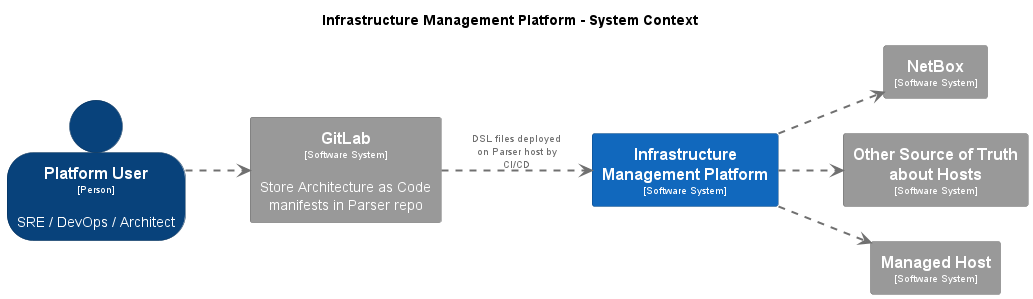
\includegraphics[width=0.95\linewidth]{../platform-arch-images/system-context.png}
  \caption{Системный контекст автоматизированной платформы управления инфраструктурой}
  \label{fig:ch2-system-context}
\end{figure}

Из рисунка~\ref{fig:ch2-system-context} видно, что платформа занимает промежуточное положение между архитектурным описанием и управляемой инфраструктурой. Она не заменяет репозиторий архитектурных артефактов и не является источником всех сведений о хостах. Ее роль состоит в связывании этих источников в один цикл управления: архитектурная модель задает целевое состояние, inventory-источники дают фактическое состояние, а reconcile-контур выполняет восстановление поддержанных workload.

\subsection{Контейнерная декомпозиция: ParserSvc, InventorySvc, DriftDetectorSvc, ReconcilerSvc}

Для реализации платформы выбрана сервисная декомпозиция. Каждый сервис отвечает за отдельную часть control loop и имеет собственный API. Такое разбиение уменьшает связность и позволяет независимо развивать источники desired state, источники actual state, алгоритмы detection и механизмы reconcile.

Контейнерная архитектура платформы представлена на рисунке~\ref{fig:ch2-container-diagram}.

\begin{figure}
  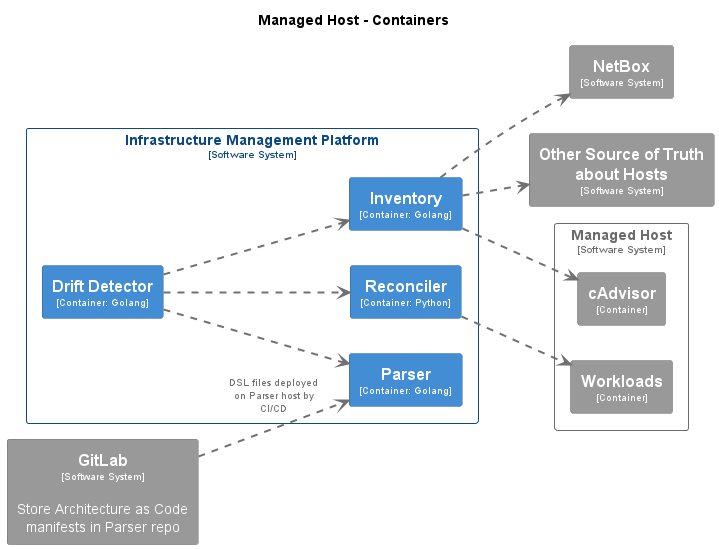
\includegraphics[width=0.95\linewidth]{../platform-arch-images/container-diagram.png}
  \caption{Контейнерная архитектура автоматизированной платформы управления инфраструктурой}
  \label{fig:ch2-container-diagram}
\end{figure}

ParserSvc отвечает за преобразование Architecture-as-Code-описания в desired state. Он выделяет deployment-узлы, свойства хостов и экземпляры контейнеров, после чего строит host-centric представление целевого состояния. ParserSvc предоставляет read-only API, через который другие сервисы могут получить полный desired state или сведения по отдельным хостам.

InventorySvc отвечает за actual state. Он загружает bootstrap-описание управляемых хостов, периодически обращается к источникам данных и формирует снимок фактического состояния. Сервис не проксирует внешний источник при каждом запросе, а обновляет внутренний snapshot и отдает его через read-only API. Такое решение снижает связанность API с доступностью внешнего источника в конкретный момент запроса.

DriftDetectorSvc является центральным компонентом цикла сравнения. Он получает desired state из ParserSvc и actual state из InventorySvc, сопоставляет хосты и применяет набор detector-ов для поддержанных workload. При обнаружении drift сервис формирует reconcile-команду и отправляет ее в ReconcilerSvc. Дополнительно DriftDetectorSvc отвечает за anti-spam/cooldown-семантику, чтобы повторяющийся drift не приводил к неограниченному числу одинаковых reconcile-запросов.

ReconcilerSvc принимает reconcile-команды и выполняет восстановление через operator-слой. Сервис реализован на Python/FastAPI и возвращает ответ \texttt{202 Accepted} после постановки задачи во внутреннюю очередь. Фактическое выполнение происходит асинхронно через Ansible Runner. Такое разделение важно, поскольку reconcile может занимать значительно больше времени, чем HTTP-запрос, и не должен блокировать DriftDetectorSvc до завершения playbook.

Контейнерная декомпозиция отражает естественное разделение данных:
\begin{enumerate}
    \item ParserSvc является источником desired state;
    \item InventorySvc является источником actual state;
    \item DriftDetectorSvc является сервисом принятия решения о drift;
    \item ReconcilerSvc является сервисом исполнения восстановительных действий.
\end{enumerate}

Такой подход также упрощает дальнейшее развитие. Например, добавление нового источника actual state требует изменения InventorySvc, но не должно менять ParserSvc. Добавление нового workload требует нового detector-а в DriftDetectorSvc и соответствующего operator-а в ReconcilerSvc, но не обязательно меняет API остальных сервисов.

\subsection{Модель desired state на основе Architecture-as-Code}

Desired state проектируется как host-centric модель. Это означает, что центральной сущностью становится хост, а требуемые workload рассматриваются как элементы, размещенные на этом хосте. Такой выбор соответствует задаче платформы: drift необходимо обнаруживать не в абстрактной архитектурной модели, а на конкретных управляемых хостах.

Входным форматом для ParserSvc является Structurizr JSON, для построения desired state используются его следующие части:
\begin{enumerate}
    \item \texttt{model.deploymentNodes} --- источник deployment-узлов, интерпретируемых как управляемые хосты;
    \item \texttt{model.softwareSystems[].containers} --- источник определений контейнеров и их имён;
    \item свойства deployment node --- источник \texttt{host\_id}, \texttt{fqdn}, \texttt{env}, \texttt{managed\_by}, \texttt{purpose} и дополнительных labels;
    \item свойства container instance --- источник признака включения workload, режима развертывания, image, version и port.
\end{enumerate}

Внутренняя модель desired state включает сущность \texttt{DesiredHost}. Для хоста обязательны \texttt{host\_id}, \texttt{fqdn}, \texttt{env}, \texttt{managed\_by}, \texttt{purpose}; поле \texttt{ip} является необязательным. Labels формируются из свойств deployment node и включают обязательные атрибуты окружения, владельца управления и назначения хоста. Такая модель позволяет в дальнейшем фильтровать хосты и группировать их по эксплуатационным признакам.

Workload в desired state описывается сущностью \texttt{DesiredWorkload}. Для MVP важны поля \texttt{name}, \texttt{enabled}, \texttt{deployment\_mode}, \texttt{image}, \texttt{version} и \texttt{port}. Поля \texttt{enabled} и \texttt{deployment\_mode} определяют, должен ли detector учитывать workload при проверке. Например, в текущей логике DriftDetectorSvc рассматривает workload только если он включен и имеет режим \texttt{container}.

С точки зрения проектирования важно, что ParserSvc не выполняет reconcile и не обращается к управляемым хостам. Его задача ограничена построением корректного snapshot desired state. Если часть манифестов некорректна, сервис должен зафиксировать ошибки, пропустить невалидные элементы и сохранить валидную часть состояния. Если ни один валидный JSON не загружен, сервис остается наблюдаемым через health endpoint, но readiness отражает отсутствие готового desired state.

Таким образом, модель desired state переводит Architecture-as-Code из уровня документации в уровень входных данных control loop. Это является ключевой особенностью платформы: архитектурная deployment-модель становится основанием для автоматизированной проверки инфраструктуры.

\subsection{Модель actual state и сбор данных через inventory}

Actual state проектируется как read-model текущего состояния управляемых хостов, он должен отражать наблюдаемое состояние инфраструктуры. Поэтому InventorySvc отделен от ParserSvc и имеет собственную модель данных, жизненный цикл синхронизации и partial-семантику.

Минимальный набор управляемых хостов задается через bootstrap-описание \texttt{selfProvisioning}. В нем указываются \texttt{id}, \texttt{fqdn} и labels хоста. Такой файл не является полноценным источником фактического состояния workload; он задает область наблюдения, то есть список хостов, по которым InventorySvc должен пытаться собрать данные.

Далее InventorySvc обращается к источникам actual state. Для каждого bootstrap-хоста сервис строит URL к cAdvisor endpoint, получает список контейнеров, нормализует ответ и преобразует его во внутреннюю модель \texttt{Workload}. Из ответа выделяются имя workload, image, runtime, источник данных и время наблюдения.

Для actual state проектируется явная модель статусов. Каждый хост может иметь статус \texttt{ok}, \texttt{partial}, \texttt{error} или \texttt{bootstrap\_only}. Дополнительно хранится \texttt{sourceStatus}: карта статусов по каждому источнику данных. Такой подход позволяет DriftDetectorSvc отличать подтвержденное отсутствие workload от отсутствия достоверных данных.

Partial result является отдельным проектным требованием. Если часть хостов или источников недоступна, InventorySvc не должен завершать работу ошибкой и не должен скрывать неполноту. Вместо этого он возвращает данные по доступным хостам и явно выставляет признаки \texttt{metadata.isPartial}, \texttt{failedHosts}, а также статусы по отдельным источникам. Такая модель повышает устойчивость платформы и снижает риск ошибочных reconcile-действий.

InventorySvc хранит actual state как in-memory snapshot. API читает уже подготовленный snapshot, а не инициирует сбор данных при каждом запросе. Это решение важно по двум причинам. Во-первых, оно отделяет частоту внешней синхронизации от частоты запросов других сервисов. Во-вторых, оно делает API-ответ согласованным: DriftDetectorSvc получает снимок состояния, сформированный в рамках завершенного цикла синхронизации.

\subsection{Сценарий drift detection и reconcile}

Основной сценарий платформы представляет собой последовательный цикл обработки. DriftDetectorSvc получает desired state от ParserSvc и actual state от InventorySvc. Далее он сопоставляет хосты, применяет detector-ы и при необходимости отправляет reconcile-команды в ReconcilerSvc.

Сопоставление хостов выполняется по \texttt{host\_id}; если оно не дает результата, используется fallback по \texttt{fqdn}. Такое решение повышает устойчивость к неполному заполнению данных, но сохраняет приоритет стабильного идентификатора. Если actual-host для desired-host не найден, ситуация фиксируется как partial, а хост пропускается. Это важно: отсутствие хоста в actual state не рассматривается как достаточное основание для автоматического восстановления всех его workload.

Detector-слой проектируется как расширяемый registry. Каждый detector отвечает за один поддерживаемый компонент и знает:
\begin{enumerate}
    \item как найти соответствующий workload в desired state;
    \item какие условия делают проверку применимой;
    \item как оценить полноту actual data;
    \item как определить drift;
    \item как сформировать reconcile-команду.
\end{enumerate}

В MVP поддержаны \texttt{node\_exporter} и \texttt{cadvisor}. Для \texttt{node\_exporter} drift означает, что workload включен в desired state, имеет режим \texttt{container}, но отсутствует в actual state при здоровом источнике cAdvisor. Для \texttt{cadvisor} дополнительно предусмотрен bootstrap-сценарий: если источник cAdvisor недоступен, сервис может инициировать установку cAdvisor, поскольку сам cAdvisor является необходимым компонентом для последующего получения actual state.

Перед отправкой reconcile-команды применяется anti-spam/cooldown-механизм. Его задача --- предотвратить повторную отправку одинаковых команд в коротком временном окне. Ключ cooldown строится по компоненту и FQDN хоста. Если для этой пары недавно уже отправлялся reconcile, повторная команда подавляется, а факт подавления фиксируется в статистике цикла.

ReconcilerSvc проектируется как асинхронный исполнитель. HTTP-запрос \texttt{POST /api/v1/reconcile} возвращает \texttt{202 Accepted}, если команда валидна и поставлена в очередь. Такой ответ означает принятие задачи, но не гарантирует успешное завершение действия на хосте. Это осознанная семантика MVP: результат выполнения фиксируется в логах, а повторная попытка может быть инициирована следующим циклом detection, если drift сохранится.

Operator-слой ReconcilerSvc отделяет API от конкретных playbook. Operator выбирает playbook и формирует execution plan, а Ansible Runner выполняет этот план на целевом хосте \cite{ansible_docs}. Такой подход сохраняет расширяемость: для нового workload необходимо добавить operator и playbook, не меняя общий API reconcile.

Сценарий drift detection и reconcile проектируется как безопасный и ограниченный. Платформа не пытается автоматически исправлять все возможные расхождения инфраструктуры. Она обнаруживает только поддержанные типы drift и выполняет только заранее определенные действия. Это соответствует природе MVP и снижает риск непредсказуемых изменений.

\subsection{Выбор технологий и границы MVP}

Технологический стек выбран исходя из задач отдельных сервисов. ParserSvc, InventorySvc и DriftDetectorSvc реализуются на Go. Этот выбор оправдан для сервисов, которым нужны компактные бинарные артефакты, простая контейнеризация, эффективная работа с HTTP API и конкурентными операциями.

ReconcilerSvc реализуется на Python/FastAPI. Этот выбор связан с естественной интеграцией Python-экосистемы с Ansible Runner. FastAPI предоставляет удобный способ описания HTTP API и валидации запросов через Pydantic, а Python позволяет напрямую использовать ansible-runner без дополнительного межъязыкового слоя.

В качестве формата Architecture-as-Code используется Structurizr JSON. Это решение связано с поддержкой C4-модели и возможностью описывать deployment-узлы и экземпляры контейнеров \cite{c4_model,structurizr_dsl}. Сервис ParserSvc читает именно JSON-представление, что уменьшает сложность реализации и делает входной контракт более явным.

cAdvisor выбран как минимальный источник actual state для контейнерных workload. Он предоставляет сведения о контейнерах на хосте, которые можно нормализовать до модели workload.

Ansible Runner выбран как механизм выполнения reconcile. Ansible хорошо подходит для agentless-доступа к хостам по SSH и для описания идемпотентных ролей установки контейнерных workload \cite{ansible_docs}. При этом сама платформа не становится ``оберткой над Ansible'': Ansible используется только внутри ReconcilerSvc как executor, а решение о drift принимается отдельным сервисом.

Границы MVP зафиксированы следующим образом:
\begin{enumerate}
    \item источник desired state --- Structurizr JSON;
    \item DSL-разбор внутри ParserSvc не выполняется;
    \item состояние сервисов хранится в памяти, persistence и история snapshot не реализованы;
    \item основной источник actual state --- cAdvisor;
    \item NetBox и другие источники рассматриваются как точки расширения;
    \item поддержанные workload --- \texttt{node\_exporter} и \texttt{cadvisor};
    \item drift-модель ограничена отсутствием требуемого контейнерного workload;
    \item результат reconcile не хранится как job history и не доступен через отдельный status API;
    \item безопасность API и аутентификация внешних вызовов находятся вне текущего MVP.
\end{enumerate}

Такие ограничения не противоречат цели работы. Напротив, они позволяют проверить основную архитектурную гипотезу: Architecture-as-Code может быть использован как источник desired state для автоматизированного управления инфраструктурой, если дополнить его inventory-слоем, drift detection и ограниченным reconcile-контуром.

Таким образом, в главе спроектирована автоматизированная платформа управления инфраструктурой с поддержкой подхода Architecture-as-Code. Определены требования, внешние участники, сервисная декомпозиция, модели desired state и actual state, сценарий drift detection/reconcile, технологический стек и границы MVP. Следующая глава посвящена реализации этих проектных решений в конкретных компонентах платформы.
